% !TEX TS-program = pdflatex
% !TEX encoding = UTF-8 Unicode

\documentclass[a4paper, titlepage=false, parskip=full-, 10pt]{scrartcl}

\usepackage[utf8]{inputenc}
\usepackage[T1]{fontenc}
\usepackage[english, ngerman]{babel}
\usepackage{babelbib}
\usepackage{hyperref}
\usepackage{listings}
\usepackage{framed}
\usepackage{color}
\usepackage{graphicx}
\usepackage[normalem]{ulem}
\usepackage{cancel}
\usepackage{amsmath}
\usepackage{amssymb}
\usepackage{amsthm}
\usepackage{algorithm}
\usepackage{algorithmic}
\usepackage{geometry}
\geometry{a4paper, top=20mm, left=35mm, right=25mm, bottom=40mm}

\newcounter{tasknbr}
\setcounter{tasknbr}{1}
\newenvironment{task}[1]{{\bf Aufgabe \arabic {tasknbr}\stepcounter{tasknbr}} (#1):\begin{enumerate}}{\end{enumerate}}
\newcommand{\subtask}[1]{\item[#1)]}

% Listings -----------------------------------------------------------------------------
\definecolor{red}{rgb}{.8,.1,.2}
\definecolor{blue}{rgb}{.2,.3,.7}
\definecolor{lightyellow}{rgb}{1.,1.,.97}
\definecolor{gray}{rgb}{.7,.7,.7}
\definecolor{darkgreen}{rgb}{0,.5,.1}
\definecolor{darkyellow}{rgb}{1.,.7,.3}
\lstloadlanguages{C++,[Objective]C,Java}
\lstset{
escapeinside={§§}{§§},
basicstyle=\ttfamily\footnotesize\mdseries,
columns=fullflexible, % typewriter font look better with fullflex
keywordstyle=\bfseries\color{blue},
% identifierstyle=\bfseries,
commentstyle=\color{darkgreen},      
stringstyle=\color{red},
numbers=left,
numberstyle=\ttfamily\scriptsize\color{gray},
% stepnumber=5,
% numberfirstline=true,
breaklines=true,
% prebreak=\\,
showstringspaces=false,
tabsize=4,
captionpos=b,
% framexrightmargin=-.2\textwidth,
float=htb,
frame=tb,
frameshape={RYR}{y}{y}{RYR},
rulecolor=\color{black},
xleftmargin=15pt,
xrightmargin=4pt,
aboveskip=\bigskipamount,
belowskip=\bigskipamount,
backgroundcolor=\color{lightyellow},
extendedchars=true,
belowcaptionskip=15pt}

%% Enter current values here: %%
\newcommand{\lecture}{Algorithmische Geometrie SS15}
\newcommand{\tutor}{}
\newcommand{\assignmentnbr}{1}
\newcommand{\students}{Julius Auer, Alexa Schlegel}
%%-------------------------------------%%

\begin{document}  
{\small \textsl{\lecture \hfill \tutor}}
\hrule
\begin{center}
\textbf{Übungsblatt \assignmentnbr}\\
[\bigskipamount]
{\small \students}
\end{center}
\hrule

\begin{task}{Geradendarstellung}
\subtask{a}
(b) geht direkt aus (c) hervor und umgekehrt, da $\overrightarrow n\cdot\overrightarrow x=n_x\cdot x_x+n_y\cdot x_y$\\
Es muss allerdings bei der Umrechnung (b)->(c) auf die Normierung von $n$ geachtet werden, so dass
$$\overrightarrow n=\frac{\begin{pmatrix}a\\b\end{pmatrix}}{\left |\begin{pmatrix}a\\b\end{pmatrix}\right |}$$

(a)->(c):\\
Steigungsvektor $\overrightarrow u$ zwischen $\overrightarrow p$ und $\overrightarrow q$ ist gegeben durch:
$$\overrightarrow u=\overrightarrow p-\overrightarrow q$$
Und somit:
$$\overrightarrow n=\frac{\begin{pmatrix}-u_y\\u_x\end{pmatrix}}{\left |\begin{pmatrix}-u_y\\u_x\end{pmatrix}\right |}$$
Sowie:
$$c=\overrightarrow p\cdot\overrightarrow n$$

(c)->(a):\\
Für Geraden, die parallel zur x-Achse verlaufen, werden zwei Punkte $p,q$ mit $p_x=0, q_x=1$ berechnet, die auf der Geraden liegen. Für alle anderen werden zwei Punkte $p,q$ mit $p_y=0, q_y=1$ berechnet:\\
\begin{align*}
p=&\begin{cases}(0,c)&\text{, falls }n_x=0\\
(\frac{c}{n_x},0)&\text{, sonst}
\end{cases}\\
q=&\begin{cases}(1,c)&\text{, falls }n_x=0\\
(\frac{c-n_y}{n_x},1)&\text{, sonst}
\end{cases}
\end{align*}

\subtask{b}
Sei $g'$ die Gerade, die parallel zu $g$ verläuft und den Punkt $p$ beinhaltet. $g'$ kann durch die folgende Normalengleichung eindeutig beschrieben werden:
\begin{align}
g'=\{\overrightarrow x\in\mathbb{R}^2|\overrightarrow n\cdot(\overrightarrow x-\overrightarrow p) = 0\}
\end{align}
Auf $g'$ liegen folglich alle Punkte $(x,y)$, mit der Eigenschaft:
\begin{align}
n_x\cdot (x-p_x)+n_y\cdot (y-p_y)=0
\end{align}
Sei $h$ die Gerade, die durch den Ursprung verläuft und senkrecht auf $g$ (und $g'$) steht. Der Normalenvektor $\overrightarrow m$ von $h$ ist dann gegeben durch:
$$\overrightarrow m=\begin{pmatrix}n_y\\-n_x\end{pmatrix}$$
Auf $h$ liegen folglich alle Punkte $(x,y)$, mit der Eigenschaft:
\begin{align}
\overrightarrow m\cdot (\overrightarrow{(x,y)}-\overrightarrow{(0,0)}&=0\\
n_y\cdot x-n_x\cdot y&=0\\
\frac{n_x\cdot y}{n_y}&=x
\end{align}
Es kann nun der Schnittpunkt $S=(x,y)$ zwischen $g'$ und $h$ berechnet werden, indem zunächst (5) in (2) eingesetzt wird um die y-Komponente zu bestimmen. Die x-Komponente ergibt sich danach analog.
\begin{align}
n_x\cdot\left( \frac{n_x\cdot y}{n_y}-p_x\right) +n_y\cdot (y-p_y)&=0\\
\frac{n_y\cdot (n_x\cdot p_x+n_y\cdot p_y)}{n_x^2+n_y^2}&=y\\
\frac{\overrightarrow n\cdot\overrightarrow p\cdot n_y}{n_x^2+n_y^2}&=y
\end{align}
Da natürlich aufgrund der Normierung $n_x^2+n_y^2=|\overrightarrow n|=1$ lässt sich dies vereinfachen zu:
\begin{align}
\overrightarrow n\cdot\overrightarrow p\cdot n_y=y\\
\overrightarrow n\cdot\overrightarrow p\cdot n_x=x
\end{align}
Die Entfernung von $S$ zum Ursprung $d$ ist nun genau der euklidische Abstand:
\begin{align}
d&=((\overrightarrow n\cdot\overrightarrow p)^2\cdot (n_x^2+n_y^2))^\frac{1}{2}\\
d&=((\overrightarrow n\cdot\overrightarrow p)^2\cdot 1)^\frac{1}{2}\\
d&=\overrightarrow n\cdot\overrightarrow p
\end{align}
Nach Definition ist die Entfernung von $g$ zum Ursprung genau $c$. Die gesuchte Entfernung $c'$ zwischen den parallelen Geraden $g$ und $g'$ - die offensichtlich genau der Entfernung von $p$ zu $g$ entspricht - ist somit gegeben durch:
\begin{align}
d&=c+c'\\
c'&=\overrightarrow n\cdot\overrightarrow p-c
\end{align}
\qed
\end{task}

\begin{task}{Implementierung}
\item[]
Grundlage für alle hier verwendeten Klassen ist eine ältere Implementierung von Matrizen, die elementare Operationen ermöglicht und - falls erforderlich - ein späteres Erweitern auf $\mathbb{R}^3$ erleichtern soll. Hierauf bauen zwei Klassen ''Point'' und ''Vector'' auf, die eine $1\times 2$ bzw. eine $2\times 1$ Matrix wrappen und diverse Operationen unterstützen. Der Code hierfür ist algorithmisch uninteressant und kann bei Bedarf im Jar eingesehen werden.

\subtask{a}
Für Geraden ist ein Konstruktor mit eingeschränkter Sichtbarkeit implementiert, der mit unterschiedlichen Geradendarstellungen aufgerufen werden kann, solange zwei Punkte auf der Gerade $p1,p2$ übergeben werden. Für gerichtete Geraden zeigt der Richtungsvektor stets von $p1$ nach $p2$. Werden nur zwei Punkte übergeben, werden alle weiteren Werte aus diesen Punkten berechnet:
\newpage
\lstset{language=Java}
\begin{lstlisting}
    /**
     * Any point on the line
     */
    final public Point  p1;

    /**
     * A point on the line, other than p1. In case of a directed line, the line
     * is directed from p1 to p2
     */
    final public Point  p2;

    /**
     * Slope of the line
     */
    final public Vector u;

    /**
     * A normal vector, orthogonal to the line
     */
    final public Vector n;

    /**
     * The normalized normal vector
     */
    final public Vector n0;

    /**
     * Distance between line and the coordinate systems center
     */
    final public double d;

    protected Line(Point p1, Point p2, Vector u, Vector n, Vector n0, double d) {
        super();
        this.p1 = p1;
        this.p2 = p2;

        if(u == null)
            // u = p1 - p2
            this.u = p2.toPosition().substract(p1.toPosition()).normalize();
        else
            this.u = u.normalize();

        if(n == null)
            // n = (-u.y, u.x)
            this.n = new Vector(-this.u.get(1), this.u.get(0));
        else
            this.n = n;

        if(n0 == null) {
            // n0 = n/|n|
            // d = - p1 * n0
            this.n0 = this.n.normalize();
            this.d = -p1.toPosition().dotProduct(this.n0);
        }
        else {
            this.n0 = n0;
            this.d = d;
        }
    }
\end{lstlisting}

\subtask{b}
\emph{getIntersection(Line line)} liefert einen Punkt zurück, oder ''null'' falls kein Schnittpunkt existiert. In diesem Fall kann mit \emph{isParallelTo(Line line)} auf Parallelität geprüft werden (für Strecken ist dies relevant, da ''null'' sowohl auf Parallelität als auch auf ''vorbeilaufen'' zurückzuführen sein kann). Die Schnittstellenberechnung löst das Gleichungssystem, in dem die Geradengleichungen der zwei Geraden gleichgesetzt werden.

\emph{C.E} ist eine Konstante (derzeit mit dem experimentell festgestellten Wert $1.0E-10d$) um beim Vergleichen von doubles eine gewisse Ungenauigkeiten zulassen zu können.
\begin{lstlisting}
public boolean isParallelTo(Line line) {
        return 1.0d - Math.abs(u.dotProduct(line.u)) < C.E;
    }

    public Point getIntersection(Line line) {
        if(isParallelTo(line))
            return null;

        double d1 = p2.getX() - p1.getX();
        double d2 = p2.getY() - p1.getY();
        double d3 = line.p2.getX() - line.p1.getX();
        double d4 = line.p2.getY() - line.p1.getY();
        double d5 = p2.getX() * p1.getY() - p1.getX() * p2.getY();
        double d6 = line.p2.getX() * line.p1.getY() - line.p1.getX() * line.p2.getY();
        double d7 = d1 * d4 - d3 * d2;
        return new Point((d3 * d5 - d1 * d6) / d7,
                (d5 * d4 - d6 * d2) / d7);
    }
\end{lstlisting}

\subtask{c}
Da der Normalenvektor vorzeichenbehaftet gespeichert wird, geht links/rechts direkt aus Einsetzen in die Normalangleichung hervor. Die Methode ist für Punkte implementiert:
\begin{lstlisting}
    /**
     * For directed lines:
     * +distance, if point is located left of the line
     * -distance, if point is located the right of the line
     * 
     * @param line a line
     * @return distance between this point and line
     */
    public double distanceTo(Line line) {
        return toPosition().dotProduct(line.n0) + line.d;
    }
\end{lstlisting}

\subtask{d}
\emph{LineSegment} ist eine Unterklasse von \emph{Line}, wobei $p1, p2$ hier die zusätzliche Funktion erfüllen, eine Strecke zu definieren. Es wird nur die Methode \emph{getIntersection(Line line)} überschrieben:
\begin{lstlisting}
    @Override
    public Point getIntersection(Line line) {
        Point is = super.getIntersection(line);

        if(is==null || !is.isInsideBoundingBox(this)
                || (line instanceof LineSegment && !is.isInsideBoundingBox((LineSegment) line)))
            return null;

        return is;
    }
\end{lstlisting}
\emph{isInsideBoundingBox(Line line)} ist hierbei eine Methode von Punkten:
\begin{lstlisting}
    public boolean isInsideBoundingBox(LineSegment ls) {
        if(getX() < Math.min(ls.p1.getX(), ls.p2.getX())
                || getX() > Math.max(ls.p1.getX(), ls.p2.getX())
                || getY() < Math.min(ls.p1.getY(), ls.p2.getY())
                || getY() > Math.max(ls.p1.getY(), ls.p2.getY()))
            return false;

        return true;
    }
\end{lstlisting}
\end{task}

\begin{task}{BHD}
\subtask{a}
Punkt in Polygon:

Eingabe ist ein Knoten eines Polygons in BHD $n$ und der zu untersuchende Punkt $p$. Jeder Knoten im Baum $n$ hat ein linkes Kind $n.left$, ein rechtes Kind $n.right$ und einen Wert in Form einer Gerade $n.line$. Für eine Gerade $g$ und einen Punkt $p$ sei \emph{dist(g,p)} der Algorithmus, der den vorzeichenbehafteten Abstand von $p$ zu $g$ berechnet, wie in Aufgabe 2 beschrieben. Initial aufgerufen wird der Algorithmus mit der Wurzel des Baumes.
\begin{algorithm}
\caption{PointInPolygon(n,p)}
\begin{algorithmic}
\IF{$n.left==null\ \AND\ n.right==null$}
\RETURN{$false$}
\ENDIF
\IF{$n.left==null\ \AND\ \NOT\ n.right==null$}
\RETURN{$PointInPolygon(n.right,p)$}
\ENDIF
\IF{$\NOT\ n.left==null\ \AND\ n.right==null$}
\RETURN{$PointInPolygon(n.left,p)$}
\ENDIF
\STATE{$leftOfLeftChild=(dist(n.left.line,p)> 0)$}
\STATE{$leftOfRightChild=(dist(n.right.line,p)> 0)$}
\IF{$leftOfLeftChild\ \AND\ leftOfRightChild$}
\RETURN{$false$}
\ENDIF
\IF{$\NOT\ leftOfLeftChild\ \AND\ \NOT\ leftOfRightChild$}
\RETURN{$true$}
\ENDIF
\IF{$leftOfLeftChild$}
\RETURN{$PointInPolygon(n.left,p)$}
\ENDIF
\RETURN{$PointInPolygon(n.right,p)$}
\end{algorithmic}
\end{algorithm}

\subtask{b}
Schnitt Gerade-Polygon:

Wenn mein Gedächtnis noch einigermaßen funktioniert wurde das in der Vorlesung nicht behandelt!?

Um Fehlerquellen beim Entwickeln eines zuvor unbekannten Algorithmus zu vermeiden wurde selbiger kurzerhand implementiert: \emph{intersectsWith(Line line)} ist eine Methode von Polygonen. In diesen wird ein BHD-Baum erzeugt, der über das Wurzelelement \emph{bHDRoot} referenziert werden kann. Noch einmal Pseudo-Code zu schreiben erscheint an dieser Stelle redundant, deshalb folgt kommentierter Java-Code:
\newpage
\lstset{language=Java}
\begin{lstlisting}
     /**
     * Search recursively for intersections of a line with the polygons hull and
     * store them in an accumulator.
     * 
     * @param line a line
     * @param node the current node of the BHD-Tree
     * @param acc an accumulator
     */
    private void intersectionWith(Line line, BHDNode node, LinkedList<Point> acc) {
        // Once only it may occur, that a linesegment is parallel to the line.
        // In this case, nothing helps but to search both branches. The same can
        // be done at root level
        if(node.line == null || node.line.isParallelTo(line)) {
            intersectionWith(line, node.left, acc);
            intersectionWith(line, node.right, acc);
            return;
        }

        // On leaf level compute intersections immediately and return
        if(node.left == null && node.right == null) {
            Point intersection = node.line.getIntersection(line);

            if(intersection != null)
                acc.add(intersection);

            return;
        }

        // The intersection of the extension of a linesegment with the line
        // gives a hint on which side the line lies. Anyways, if a linesegment
        // itself intersects with the line, the matching branch must always be
        // searched
        Point intersection_extendedLine = new Line(node.line.p1, node.line.p2).getIntersection(line);

        if(node.left.line.getIntersection(line) != null || intersection_extendedLine.distanceTo(node.left.line) > C.E)
            intersectionWith(line, node.left, acc);

        if(node.right.line.getIntersection(line) != null || intersection_extendedLine.distanceTo(node.right.line) > C.E)
            intersectionWith(line, node.right, acc);
    }

    public LineSegment intersectionWith(Line line) {
        LinkedList<Point> acc = new LinkedList<Point>();
        intersectionWith(line, bHDRoot, acc);

        if(acc.size() > 2)
            throw new RuntimeException("WTF: found more than 2 intersections");

        // The line passes the polygon
        if(acc.isEmpty())
            return null;

        // The line intersects the polygon. If it intersects in only one point
        // p, the line p->p is returned
        return new LineSegment(acc.getFirst(), acc.size() > 1 ? acc.get(1) : acc.getFirst());
    }
\end{lstlisting}
\newpage
Hier noch die Ausgabe einer kleinen Test-Routine:
\begin{figure}[htpb]
\begin{center}
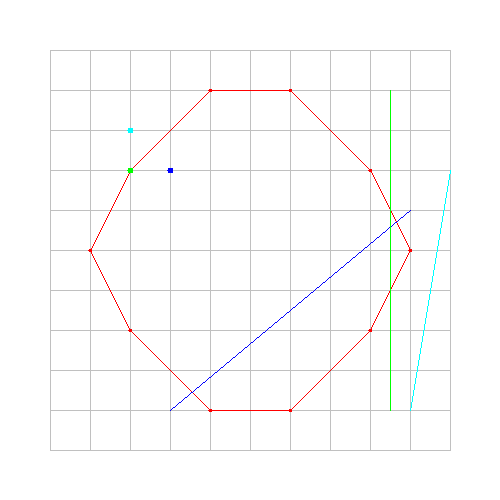
\includegraphics[width=10cm]{test}
\end{center}
\caption{Ein paar Testfälle}
\end{figure}

\framebox{\parbox{\linewidth}{
polygon contains (3.0, 7.0) (blue): true\\
polygon contains (2.0, 7.0) (green): true\\
polygon contains (2.0, 8.0) (cyan): false\\
intersection of polygon and line1 (blue): LineSegment: (8.6, 5.7) -> (3.5, 1.5)\\
intersection of polygon and line2 (green): LineSegment: (8.5, 6.0) -> (8.5, 4.0)\\
intersection of polygon and line3 (cyan): null
}}
\end{task}
\end{document}